%!TEX root = edance.tex
%%%%%%%%%%%%%%%%
%  CHAPTER 18  %
%%%%%%%%%%%%%%%%
\chapter{Non-Ideal Operational Amplifiers}
\label{ch:ch18_opamp_real}
\graphicspath{{./figures/figs_ch18_opamp_real/}}
%%%%%%%%%%%%%%%%%%%%%%%%%%%%%%%%%%%%%%%%%%%%%%%%%%%%%%%%%%%%%%%%%%%%%%%%%%%%%%%%%%%%%%%%
%%%%%%%%%%%%%%%%%%%%%%%%%%%%%%%%%%%%%%%%%%%%%%%%%%%%%%%%%%%%%%%%%%%%%%%%%%%%%%%%%%%%%%%%
%                                   SECTION 18.1                                       %
%%%%%%%%%%%%%%%%%%%%%%%%%%%%%%%%%%%%%%%%%%%%%%%%%%%%%%%%%%%%%%%%%%%%%%%%%%%%%%%%%%%%%%%%
%%%%%%%%%%%%%%%%%%%%%%%%%%%%%%%%%%%%%%%%%%%%%%%%%%%%%%%%%%%%%%%%%%%%%%%%%%%%%%%%%%%%%%%%
\section{Chapter Preview}
In the last chapter we introduced a model for an operational amplifier (op-amp) that could predict the gain-bandwidth (GBW) trade-off of the amplifier in single-pole dominated op-amps.  The model was physically inspired, and included an input OTA followed by an optional buffer.  The model accounted for finite open-loop gain ($A_0 < \infty$ ), finite input resistance ($R_i < \infty\Omega$ ), non-zero output resistance ($R_o > 0\Omega$), and finite bandwidth.

In this chapter we continue our investigation of op-amps, but we will also discuss other non-ideal effects and non-linearities that are present in real op-amps.  These include an offset voltage, DC bias currents at the input, swing and slew-rate limitations, and distortion.  We end the chapter by discussing some other effects such as noise, but we will only scratch the surface of this topic and leave this for a more advanced analog circuits course.
%%%%%%%%%%%%%%%%%%%%%%%%%%%%%%%%%%%%%%%%%%%%
%                 FIGURE                   %
%%%%%%%%%%%%%%%%%%%%%%%%%%%%%%%%%%%%%%%%%%%%
% \begin{figure}[H]
% \centering
% \includegraphics[scale=1.00]{null}
% \caption{null}
% \label{fig:ch18_intro}
% \end{figure}
%%%%%%%%%%%%%%%%%%%%%%%%%%%%%%%%%%%%%%%%%%%%
\newpage
%%%%%%%%%%%%%%%%%%%%%%%%%%%%%%%%%%%%%%%%%%%%
%                 FIGURE                   %
%%%%%%%%%%%%%%%%%%%%%%%%%%%%%%%%%%%%%%%%%%%%
\begin{figure}[tb]
\centering
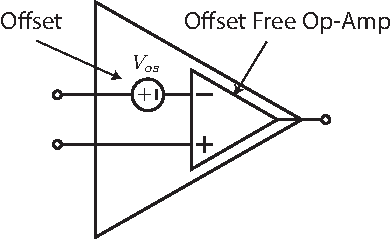
\includegraphics[scale=1.15]{opamp_offset}
\caption{The offset voltage of an op-amp can be modeled by assuming the op-amp is free of offset, and then placing a voltage source at one of the input terminals.  Since the sign of the offset voltage is a random variable, the offset voltage can be placed at either input terminal.}
\label{fig:opamp_offset}
\end{figure}
%%%%%%%%%%%%%%%%%%%%%%%%%%%%%%%%%%%%%%%%%%%%%%%%%%%%%%%%%%%%%%%%%%%%%%%%%%%%%%%%%%%%%%%%
%%%%%%%%%%%%%%%%%%%%%%%%%%%%%%%%%%%%%%%%%%%%%%%%%%%%%%%%%%%%%%%%%%%%%%%%%%%%%%%%%%%%%%%%
%                                   SECTION 18.2                                       %
%%%%%%%%%%%%%%%%%%%%%%%%%%%%%%%%%%%%%%%%%%%%%%%%%%%%%%%%%%%%%%%%%%%%%%%%%%%%%%%%%%%%%%%%
%%%%%%%%%%%%%%%%%%%%%%%%%%%%%%%%%%%%%%%%%%%%%%%%%%%%%%%%%%%%%%%%%%%%%%%%%%%%%%%%%%%%%%%%
\section{Offset Voltage and Currents}
%%%%%%%%%%%%%%%%%%%%%%%%%%%%%%%%%%%%%%%%%%%%
%             SUBSECTION 18.2.1            %
%%%%%%%%%%%%%%%%%%%%%%%%%%%%%%%%%%%%%%%%%%%%
\subsection{Offset Voltage}
If you short the inputs of an op-amp, you would expect that the output would be at zero voltages.  Unfortunately, due to imbalances in the construction of the amplifier, the output may not be at zero at all.  In fact, in many cases it might even "rail out", and sit at either $V_{sup}$ or $-V_{sup}$, where $\pm V_{sup}$ are the supply rails.  From our study of the \textit{differential pair}\index{Differential pair}, we know that the origin of this \textbf{offset voltage}\index{Op-amp!offset voltage} arises from mismatches between the input differential pair transistors or load resistors.  

We model an op-amp with an offset voltage as an ideal op-amp inside another amplifier with a simple DC offset voltage, shown in \emph{Fig.~\ref{fig:opamp_offset}}.  Even though the DC offset voltage is shown with a certain polarity, in reality it can be positive or negative, because it is a random variable.  This means that for each model of an op-amp there will be a different offset voltage for each part.  In datasheets for op-amps you will see that the stated offset voltage $V_{os}$ is usually the standard deviation of the offset voltage.  Therefore it is clear that we can place the DC voltage on either terminal.  The impact is to shift the transfer curve left or right (shown in \emph{Fig.~\ref{fig:opamp_offset_plot}}), depending on the sign and magnitude of the offset.
%%%%%%%%%%%%%%%%%%%%%%%%%%%%%%%%%%%%%%%%%%%%
%                 FIGURE                   %
%%%%%%%%%%%%%%%%%%%%%%%%%%%%%%%%%%%%%%%%%%%%
\begin{figure}[H]
\centering
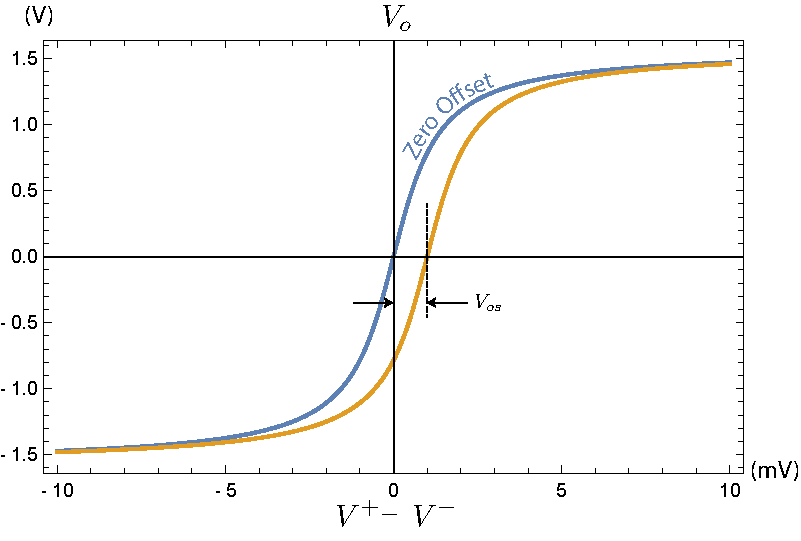
\includegraphics[width=.75\columnwidth]{opamp_offset_plot}
\caption{The offset voltage causes the input-output transfer curve of an op-amp to deviate from the origin.  In other words, even a zero input results in a non-zero output voltage.}
\label{fig:opamp_offset_plot}
\end{figure}
%%%%%%%%%%%%%%%%%%%%%%%%%%%%%%%%%%%%%%%%%%%%
\newpage
%%%%%%%%%%%%%%%%%%%%%%%%%%%%%%%%%%%%%%%%%%%%
%             SUBSECTION 18.2.2            %
%%%%%%%%%%%%%%%%%%%%%%%%%%%%%%%%%%%%%%%%%%%%
\subsection{Trimming of Offset Voltage}
%%%%%%%%%%%%%%%%%%%%%%%%%%%%%%%%%%%%%%%%%%%%
%                 FIGURE                   %
%%%%%%%%%%%%%%%%%%%%%%%%%%%%%%%%%%%%%%%%%%%%
\begin{figure}[tb]
\centering
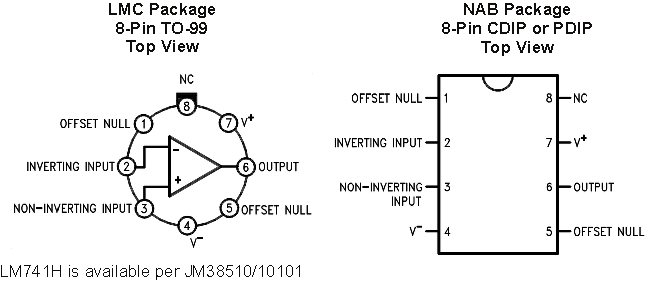
\includegraphics[width=.75\columnwidth]{lm741_pinout}
\caption{The pinout of the LM741H op-amp has several pins dedicated for offset nulling the amplifier.} \label{fig:lm741_pinout}
\end{figure}
The pinout of a typical op-amp is shown in \emph{Fig.~\ref{fig:lm741_pinout}}.  In addition to the obvious pins (input, output, supplies), there are extra pins labeled "offset null".   The output DC offset voltage of an op-amp can be trimmed to zero by connecting a potentiometer to the two offset-nulling terminals, as shown in \emph{Fig.~\ref{fig:opamp_pinout_offset}}. In this example, the wiper of the potentiometer should be connected to the negative supply of the op-amp.  In fully integrated circuits, the offset null circuitry is internal (for example with electronically steerable resistors or current sources) and the offset is nulled out using a calibration step or feedback.  
%%%%%%%%%%%%%%%%%%%%%%%%%%%%%%%%%%%%%%%%%%%%
%                 FIGURE                   %
%%%%%%%%%%%%%%%%%%%%%%%%%%%%%%%%%%%%%%%%%%%%
\begin{figure}[H]
\centering
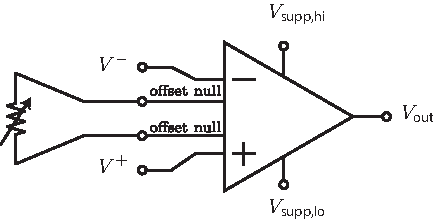
\includegraphics[scale=1.25]{opamp_pinout_offset}
\caption{The pinout of many op-amps include offset null pins that should be connected as directed in the datasheet.  For example, in this amplifier a potentiometer is used to tune out the offset.} \label{fig:opamp_pinout_offset}
\end{figure}
%%%%%%%%%%%%%%%%%%%%%%%%%%%%%%%%%%%%%%%%%%%%
%             SUBSECTION 18.2.3            %
%%%%%%%%%%%%%%%%%%%%%%%%%%%%%%%%%%%%%%%%%%%%
\subsection{Input Bias Currents and Offset Currents}
%%%%%%%%%%%%%%%%%%%%%%%%%%%%%%%%%%%%%%%%%%%%
%                 FIGURE                   %
%%%%%%%%%%%%%%%%%%%%%%%%%%%%%%%%%%%%%%%%%%%%
\begin{figure}[tb]
\centering
\begin{tabular}{cc}
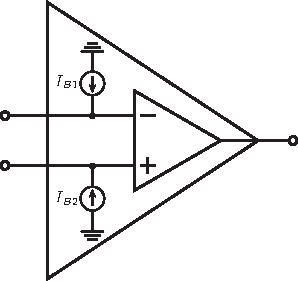
\includegraphics[scale=1.05]{opamp_offset_I} &
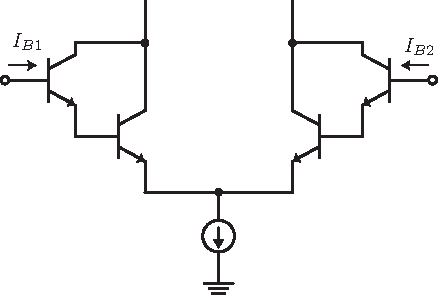
\includegraphics[scale=1.05]{bjt_input_darlington}\\
(a) & (b)\\
\end{tabular}
\caption{(a) Many op-amps require input bias currents to flow into the amplifier.  These bias currents are never perfectly matched, resulting in an input offset current. (b) The physical implementation of the input of an op-amp with bipolar transistors may incorporate a "Darlington Pair" to reduce the input current. The pair of transistors acts like a macro transistor with reduced base current. The first (input) BJT's are followers and the differential pair is formed as usual using the Darlingtons.}
\label{fig:opamp_offset_I}
\end{figure}
%%%%%%%%%%%%%%%%%%%%%%%%%%%%%%%%%%%%%%%%%%%%
Some op-amps, in particular ones implemented with bipolar transistors, have an input bias current that needs to flow into or out of the op-amp inputs in order for everything to function properly. This is typically a very small current ($100\,nA$), and modeled by adding explicit current sources to the input of an ideal op-amp, shown in \emph{Fig.~\ref{fig:opamp_offset_I}}.  The bias currents flowing into each input terminal can also vary, and the difference is the \textbf{input offset current}\index{Op-amp!input offset current}, usually an order of magnitude smaller than the input currents ($10\,nA$).  The average current is given by:
\begin{equation}
       I_B = \frac{I_{B1} + I_{B2}}{2}
\end{equation}
The difference between the bias currents is known as the offset current:
\begin{align}
        \Aboxed{I_{OS} = \left|I_{B1} - I_{B2}\right|}
        &\textit{Op-amp input offset current}
\end{align}
It is important to understand that this is a DC current.  It is \textit{not} an AC current, and it is \textit{not} due to the input impedance.  It is usually the base current of a bipolar transistor, $I_B = I_C/\beta$.  Variations in $\beta$ cause the input offset.
%%%%%%%%%%%%%%%%%%%%%%%%%%%%%%%%%%%%%%%%%%%%
%             SUBSECTION 18.2.4            %
%%%%%%%%%%%%%%%%%%%%%%%%%%%%%%%%%%%%%%%%%%%%
\subsection{Effect of Input Bias Current in Amplifier Circuit}
Let's assume for now that the offset voltage of an op-amp is zero.  In absence of an input voltage, as shown in \emph{Fig.~\ref{fig:opamp_offset_i2v}}, one would expect zero output.  However, due to non-zero $I_B$, the output is given by:
\begin{equation}
      V_o = I_{B1}\,R_2 \approx I_B\,R_2 
      \label{eq:off1}
\end{equation}
This places a limit on the value of $R_2$. A lower value of $R_2$ requires a higher power op-amp, which is undesirable in many applications.  In the next section, we will show a simple way to mitigate this.
%%%%%%%%%%%%%%%%%%%%%%%%%%%%%%%%%%%%%%%%%%%%
%                 FIGURE                   %
%%%%%%%%%%%%%%%%%%%%%%%%%%%%%%%%%%%%%%%%%%%%
\begin{figure}[H]
\centering
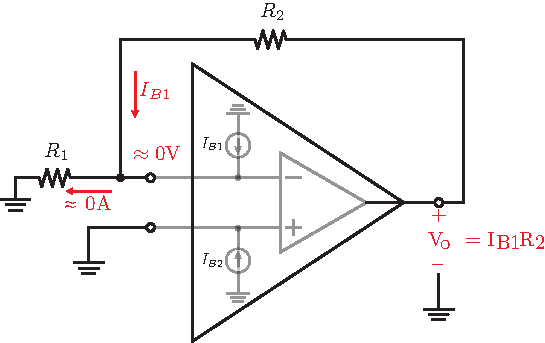
\includegraphics[scale=1.25]{opamp_offset_i2v}
\caption{In an op-amp with feedback, the input bias currents cause output offset voltages as shown.  Note the current through $R_1$ is zero since the input of the op-amp is at a virtual ground due to the high loop gain.}
\label{fig:opamp_offset_i2v}
\end{figure}
%%%%%%%%%%%%%%%%%%%%%%%%%%%%%%%%%%%%%%%%%%%%
\newpage
%%%%%%%%%%%%%%%%%%%%%%%%%%%%%%%%%%%%%%%%%%%%
%                 FIGURE                   %
%%%%%%%%%%%%%%%%%%%%%%%%%%%%%%%%%%%%%%%%%%%%
\begin{figure}[t]
\centering
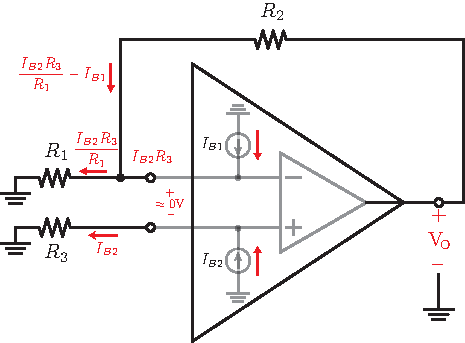
\includegraphics[scale=1.5]{opamp_offset_reduce}
\caption{The effect of input currents and input offset can be minimized by placing an appropriately sized resistor $R_3$ at the positive terminal of the op-amp without impacting the AC performance.} \label{fig:opamp_offset_reduce}
\end{figure}
%%%%%%%%%%%%%%%%%%%%%%%%%%%%%%%%%%%%%%%%%%%%
%             SUBSECTION 18.2.5            %
%%%%%%%%%%%%%%%%%%%%%%%%%%%%%%%%%%%%%%%%%%%%
\subsection{Reducing the Effect of Input Bias Currents}
In \emph{Fig.~\ref{fig:opamp_offset_reduce}}, we add a resistor $R_3$, which has no impact on the AC response of an ideal op-amp since the current into the grounded node of the positive terminal is zero.  Let's calculate the output offset voltage in this case.  The figure labels are very helpful in deriving this equation:
    \begin{equation}
          V_o = I_{B2}\,R_3 + R_2\left(\frac{I_{B2}\,R_3}{R_1} - I_{B1}\right)
    \end{equation}
Let's assume zero offset for now ($I_{B1} = I_{B2} = I_B$).  Then this equation can be simplified:
    \begin{equation}
        V_o = I_B\,R_3 + R_2\,I_B\left(\frac{R_3}{R_1} - 1\right)
    \end{equation}
The output offset voltage due to $I_B$ is given by:
    \begin{align}
        \Aboxed{V_{OS} &= I_B\left[-R_2 + R_3\left(1 + \frac{R_2}{R_1}\right)\right]}
        &\textit{Op-amp output offset voltage}
        \label{eq:op_amp_output_offset}
    \end{align}
Notice that if we choose $R_3 = \frac{R_2}{1 + R_2/R_1}$, we can drive $V_o = 0\,V$, thus eliminating the systematic offset of the circuit.  You can show that if we now include an offset current, the above choice of $R_3$ results in $V_o = I_{OS}\,R_2 $, which is an order of magnitude lower than $I_B\,R_2$ from \emph{Eq.~\ref{eq:off1}}.
\newpage
%%%%%%%%%%%%%%%%%%%%%%%%%%%%%%%%%%%%%%%%%%%%%%%%%%%%%%%%%%%%%%%%%%%%%%%%%%%%%%%%%%%%%%%%
%%%%%%%%%%%%%%%%%%%%%%%%%%%%%%%%%%%%%%%%%%%%%%%%%%%%%%%%%%%%%%%%%%%%%%%%%%%%%%%%%%%%%%%%
%                                   SECTION 18.3                                       %
%%%%%%%%%%%%%%%%%%%%%%%%%%%%%%%%%%%%%%%%%%%%%%%%%%%%%%%%%%%%%%%%%%%%%%%%%%%%%%%%%%%%%%%%
%%%%%%%%%%%%%%%%%%%%%%%%%%%%%%%%%%%%%%%%%%%%%%%%%%%%%%%%%%%%%%%%%%%%%%%%%%%%%%%%%%%%%%%%
\section{Op-Amp Frequency Response}
In the last chapter, we discussed the op-amp frequency response in detail. This section is mostly a review.  We will analyze an inverting amplifier circuit and show that our results from feedback analysis approximately hold true in this case.
%%%%%%%%%%%%%%%%%%%%%%%%%%%%%%%%%%%%%%%%%%%%
%             SUBSECTION 18.3.1            %
%%%%%%%%%%%%%%%%%%%%%%%%%%%%%%%%%%%%%%%%%%%%
\subsection{Frequency Response of Open-Loop Op-Amp}
We know from the previous chapter that op-amps are designed to have a single dominant pole.  The transfer function of the op-amp is therefore approximately given by
    \begin{equation} 
        A(j\omega) = \frac{A_0}{1 + j\omega/\omega_\text{-3dB}} 
    \end{equation}
where the DC gain is $A_0$, and the 3-dB frequency is $\omega_{\text{-3dB}}$.  We also derived the unity-gain bandwidth, $\omega_u = A_0 \omega_{\text{-3dB}}$, also known as the  gain-bandwidth product $GBW$.  For high frequencies, $\omega \gg \omega_{\text{-3dB}}$
    \begin{equation}
        A(j\omega) = \frac{\omega_u}{j\omega}
    \end{equation}
The single pole response with a dominant pole at $\omega_{\text{-3dB}}$.
%%%%%%%%%%%%%%%%%%%%%%%%%%%%%%%%%%%%%%%%%%%%
%             SUBSECTION 18.3.2            %
%%%%%%%%%%%%%%%%%%%%%%%%%%%%%%%%%%%%%%%%%%%%
\subsection{Frequency Response of Closed-Loop Op-Amp}
%%%%%%%%%%%%%%%%%%%%%%%%%%%%%%%%%%%%%%%%%%%%
%                 FIGURE                   %
%%%%%%%%%%%%%%%%%%%%%%%%%%%%%%%%%%%%%%%%%%%%
\begin{figure}[tb]
\centering
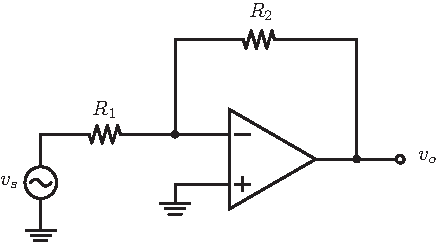
\includegraphics[scale=1]{opamp_invert_gain}
\caption{An inverting op-amp with finite gain and a single dominant pole.}
\label{fig:opamp_invert_gain}
\end{figure}
%%%%%%%%%%%%%%%%%%%%%%%%%%%%%%%%%%%%%%%%%%%%
Let's analyze the frequency response of the op-amp circuit shown in \emph{Fig.~\ref{fig:opamp_invert_gain}}.  This is a closed-loop system, so we expect the feedback analysis to hold.  Let's find the transfer function assuming finite gain $A$
    \begin{equation}
        G = \frac{v_o}{v_s} = \left(-\frac{R_2}{R_1}\right) \frac{1}{1 + (1+R_2/R_1)/A}
    \end{equation}
As expected, if $A \rightarrow \infty$, we get the transfer function for an inverting amplifier.  Now  substitute $A$ with a single-pole transfer function to obtain:
    \begin{equation} 
        A(j\omega) = \frac{A_0}{1 + j\omega/\omega_{\text{-3dB}}}
    \end{equation}
and simplify the expression 
    \begin{equation}
        G(j\omega) = \left(-\frac{R_2}{R_1}\right)  \frac{1}{1 + (1+R_2/R_1)(1+ j\omega/\omega_\text{-3dB})/A_0}
    \end{equation}
The derived transfer function can be approximated if the DC gain $A_0$ is very large:
    \begin{equation}
        G(j\omega) = \left(-\frac{R_2}{R_1}\right)  \frac{1}{1 + \frac{1+R_2/R_1}{A_0} + \frac{j\omega}{\left( \frac{A_0 \omega_\text{-3dB}}{1 + R_2/R_1} \right)}} \approx \left(-\frac{R_2}{R_1}\right)\frac{1}{1 + \frac{j\omega}{\left( \frac{A_0 \omega_\text{-3dB}}{1 + R_2/R_1} \right)}}
    \end{equation}
The closed-loop bandwidth is higher than the open-loop bandwidth (as expected from last chapter):
    \begin{equation} 
        \omega_{0} = \frac{A_0 \omega_{\text{-3dB}}}{ 1 + R_2/R_1} 
    \end{equation}
The gain-bandwidth product remains (nearly) unchanged:
    \begin{equation} 
        G \times BW = \frac{R_2}{R_1} \frac{A_0 \omega_\text{-3dB}}{ 1 + R_2/R_1} \approx \frac{R_2}{R_1} \cdot \frac{A_0 \omega_\text{-3dB}}{R_2/R_1} = A_0 \omega_\text{-3dB} = \omega_u
    \end{equation}
The closed loop transfer function in relation to the open-loop transfer function is shown in \emph{Fig.~\ref{fig:mag1pole_fb_label}}.  If you're curious why the feedback analysis did not match our previous chapter results exactly, the explanation is a bit complicated but to summarize, the inverting amplifier is not a voltage amplifier but really a current to voltage (trans-resistance) amplifier.  To see this, note that the output voltage is not subtracted from the input, since the input is also supplied at the negative op-amp terminal. The output voltage is converted to a current through $R_2$ and it's subtracted from the input current at the inverting terminal (do a Norton transformation of the source with $R_1$).
%%%%%%%%%%%%%%%%%%%%%%%%%%%%%%%%%%%%%%%%%%%%
%                 FIGURE                   %
%%%%%%%%%%%%%%%%%%%%%%%%%%%%%%%%%%%%%%%%%%%%
\begin{figure}[tb]
\centering
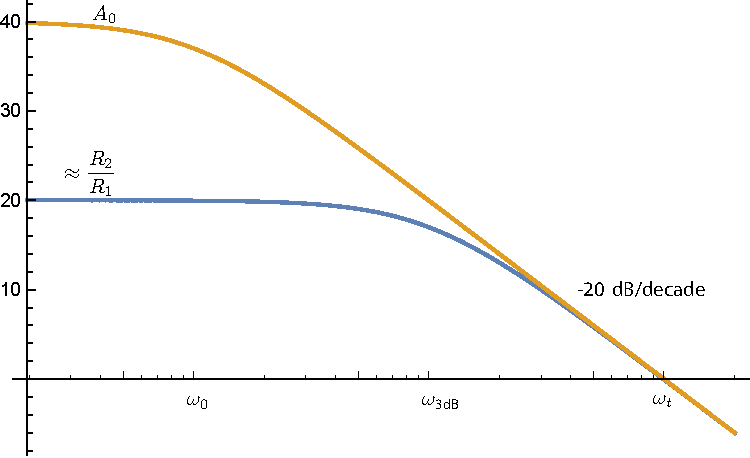
\includegraphics[scale=1]{mag1pole_fb_label}
\caption{Transfer function of op-amp based inverting amplifier in open-loop and closed-loop configuration.}
\label{fig:mag1pole_fb_label}
\end{figure}
%%%%%%%%%%%%%%%%%%%%%%%%%%%%%%%%%%%%%%%%%%%%%%%%%%%%%%%%%%%%%%%%%%%%%%%%%%%%%%%%%%%%%%%%
%%%%%%%%%%%%%%%%%%%%%%%%%%%%%%%%%%%%%%%%%%%%%%%%%%%%%%%%%%%%%%%%%%%%%%%%%%%%%%%%%%%%%%%%
%                                   SECTION 18.4                                       %
%%%%%%%%%%%%%%%%%%%%%%%%%%%%%%%%%%%%%%%%%%%%%%%%%%%%%%%%%%%%%%%%%%%%%%%%%%%%%%%%%%%%%%%%
%%%%%%%%%%%%%%%%%%%%%%%%%%%%%%%%%%%%%%%%%%%%%%%%%%%%%%%%%%%%%%%%%%%%%%%%%%%%%%%%%%%%%%%%
\section{Voltage Swing and Slewing }
%%%%%%%%%%%%%%%%%%%%%%%%%%%%%%%%%%%%%%%%%%%%
%             SUBSECTION 18.4.1            %
%%%%%%%%%%%%%%%%%%%%%%%%%%%%%%%%%%%%%%%%%%%%
\subsection{Output Saturation}
The output voltage swing is limited by the voltage supplies, usually omitted from the schematic, but shown explicitly in \emph{Fig.~\ref{fig:opamp_invert_gain_supplies}}.  If the input voltage times the gain of the amplifier is larger than the supplies, the output will clip, as shown in \emph{Fig.~\ref{fig:sin_clip}}.  Here we are optimistically assuming the op-amp can swing all the way to the rails.  In reality, the output swing may be lower than the rails due to the various implementation details.  Most op-amps also have a maximum output current limit, activated to prevent the op-amp from damage in the case of a short circuit or connection of a very small load resistor.  In either case, the output waveform will appear "clipped", leading to distortion.  In most linear amplifier applications, clipping is unwanted and avoided by careful design.
%%%%%%%%%%%%%%%%%%%%%%%%%%%%%%%%%%%%%%%%%%%%
%                 FIGURE                   %
%%%%%%%%%%%%%%%%%%%%%%%%%%%%%%%%%%%%%%%%%%%%
\begin{figure}[tb]
\centering
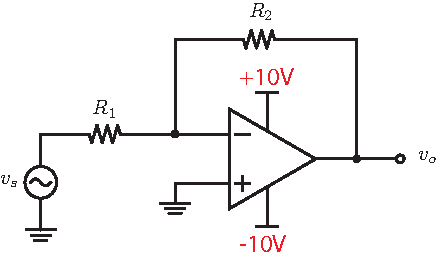
\includegraphics[scale=1]{opamp_invert_gain_supplies}
\caption{The positive and negative supplies of the op-amp are highlighted.  If the output voltage exceeds the rails, the output clips.  Usually the output cannot swing all the way to the rails, and so the output swing is even lower.}
\label{fig:opamp_invert_gain_supplies}
\end{figure}
%%%%%%%%%%%%%%%%%%%%%%%%%%%%%%%%%%%%%%%%%%%%
%                 FIGURE                   %
%%%%%%%%%%%%%%%%%%%%%%%%%%%%%%%%%%%%%%%%%%%%
\begin{figure}[tb]
\centering
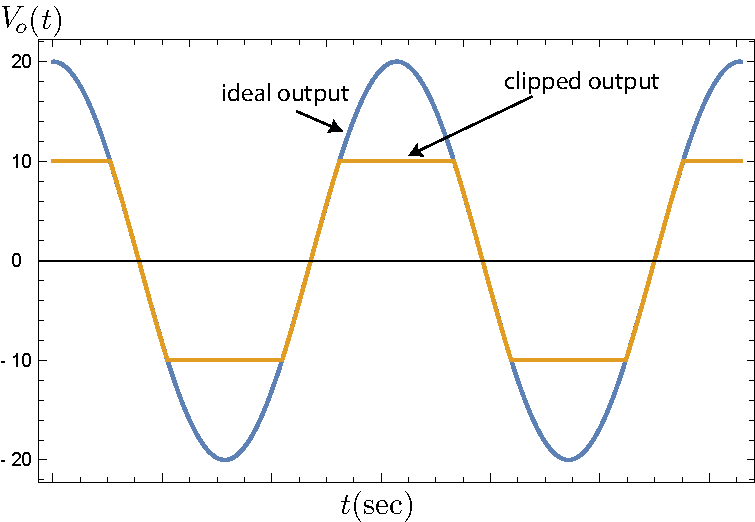
\includegraphics[width=.75\columnwidth]{sin_clip}
\caption{A large amplitude sine wave is clipped because the voltage exceeds the op-amp rails (supplies).}
\label{fig:sin_clip}
\end{figure}
%%%%%%%%%%%%%%%%%%%%%%%%%%%%%%%%%%%%%%%%%%%%
%             SUBSECTION 18.4.2            %
%%%%%%%%%%%%%%%%%%%%%%%%%%%%%%%%%%%%%%%%%%%%
\subsection{Slew Rate}
The "slew rate'', or the maximum possible change at the output, is defined by:
    \begin{equation}
        SR = \left. \frac{dV_o}{dt} \right|_{maximum}
    \end{equation}
and is usually specified in data sheets in units of $V/\mu$s.  It's very important to understand the difference between $SR$ limiting and the $BW$ limit.  The limited bandwidth is a linear phenomenon, and it does not distort the shape of a sinusoidal input.  On the other hand, $SR$ limitation can cause non-linear distortion resulting in a non-sinusoidal output waveform.
%%%%%%%%%%%%%%%%%%%%%%%%%%%%%%%%%%%%%%%%%%%%
%                 FIGURE                   %
%%%%%%%%%%%%%%%%%%%%%%%%%%%%%%%%%%%%%%%%%%%%
\begin{figure}[tb]
\centering
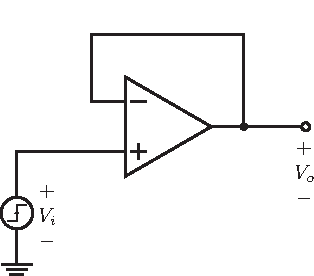
\includegraphics[scale=1]{opamp_unitygain_step}
\caption{An op-amp in unity gain configuration is driven by a step function.}
\label{fig:opamp_unitygain_step_fig}
\end{figure}
%%%%%%%%%%%%%%%%%%%%%%%%%%%%%%%%%%%%%%%%%%%%
%                 FIGURE                   %
%%%%%%%%%%%%%%%%%%%%%%%%%%%%%%%%%%%%%%%%%%%%
\begin{figure}[tb]
\centering
\begin{tabular}{cc}
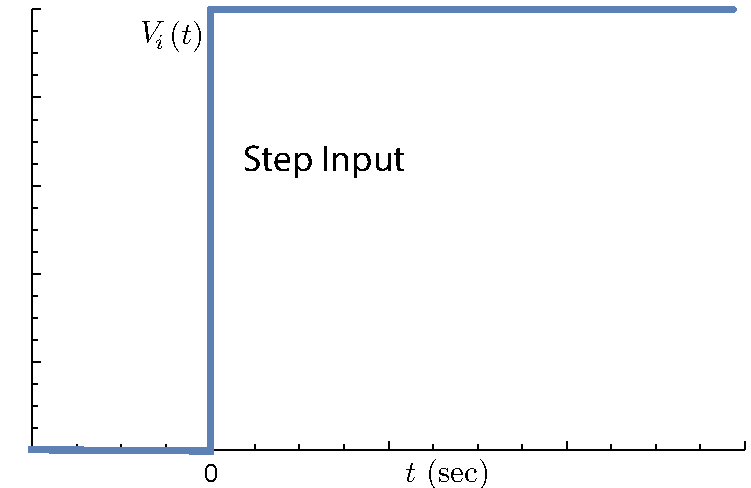
\includegraphics[width=.45\columnwidth]{step_input} &
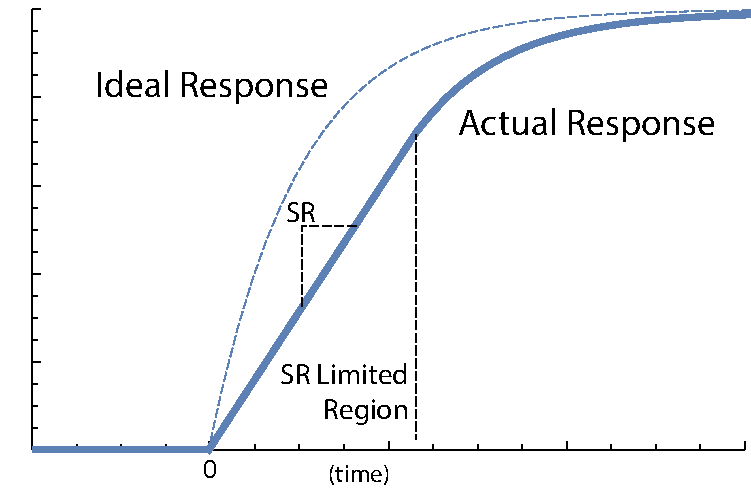
\includegraphics[width=.45\columnwidth]{exp_slew}\\
(a) & (b)\\
\end{tabular}
\caption{(a) The input step function is applied at time $t=0$s.  (b) Ideally, the output would approach the input with an exponential response and time constant commensurate inversely with the bandwidth of the amplifier. In practice, if the step is sufficiently large, the amplifier experiences slew rate limiting.}
\label{fig:step_input}
\end{figure}
%%%%%%%%%%%%%%%%%%%%%%%%%%%%%%%%%%%%%%%%%%%%
To understand SR limiting, let's consider a simple unity-gain op-amp amplifier shown in \emph{Fig.~\ref{fig:opamp_unitygain_noise_fig}}.  If a step voltage is supplied at the input, the output would ideally  follow the exponential settling predicted by simple linear theory:
    \begin{equation}
        V_o(t) = V_i \left( 1 - e^{-t \omega_u} \right) 
    \end{equation}
In this case the time constant $\tau = 1/\omega_u$ as the amplifier bandwidth is the full $GBW$ product, since it's a unity gain configuration feedback amplifier.  This settling behavior is shown in the dashed line of \emph{Fig.~\ref{fig:step_input}}.  What is surprising is that a real op-amp will not follow this linear step response, but rather a curve that is a linear ramp for a duration, labeled as the SR limited region, and then only after the slope of the waveform is small enough does the circuit behave similar the bandwidth limited case.  Essentially, the SR limit prevents the amplifier from changing faster than the slew rate.  For the linear response, the  slope of the output signal ("slew rate") is given by
    \begin{equation}
        \frac{dV_{o}}{dt} = V_i \omega_u e^{-t \omega_u}
    \end{equation}
Notice that the slope is initially the largest and given by
    \begin{equation}
        \left. \frac{dV_{o}}{dt} \right|_{\text{max}} = V_i \omega_u
    \end{equation}
and over time the slope decays. If this slope is larger than the slew rate, $V_i \omega_u > SR$, the amplifier will slew as shown in \emph{Fig.~\ref{fig:SR_case1}}.  Since this expression involves the input amplitude, it's possible to apply a smaller signal step $V_{sm,i}$ to the input and not experience any slewing, as shown in \emph{Fig.~\ref{fig:SR_case2}}:  
    \begin{equation}
        \left. \frac{dV_{o}}{dt} \right|_{\text{max}} = V_{sm,i} \omega_u  < SR
    \end{equation}
%%%%%%%%%%%%%%%%%%%%%%%%%%%%%%%%%%%%%%%%%%%%
%                 FIGURE                   %
%%%%%%%%%%%%%%%%%%%%%%%%%%%%%%%%%%%%%%%%%%%%
\begin{figure}[tb]
\centering
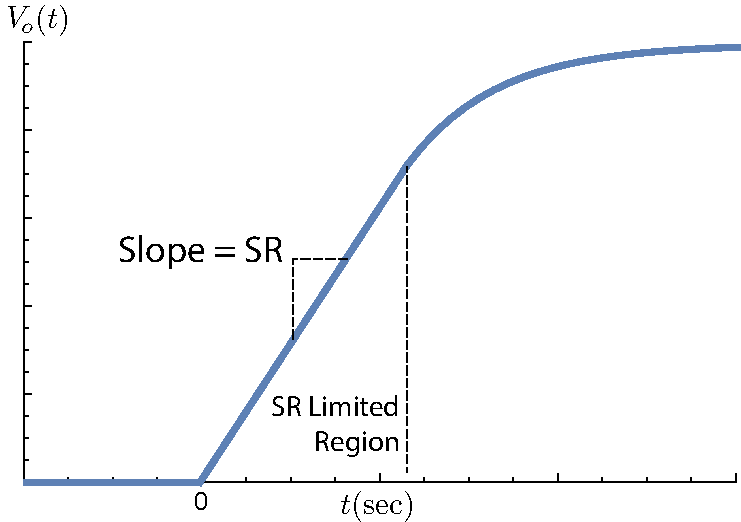
\includegraphics[width=.65\columnwidth]{SR_case1}
\caption{When an op-amp is experiencing the slew-rate limiting, the rate of change of the output is constrained to be lower than the SR limit.  In other words, the slope of the output cannot exceed $SR$.} \label{fig:SR_case1}
\end{figure} 
%%%%%%%%%%%%%%%%%%%%%%%%%%%%%%%%%%%%%%%%%%%%
%                 FIGURE                   %
%%%%%%%%%%%%%%%%%%%%%%%%%%%%%%%%%%%%%%%%%%%%
\begin{figure}[tb]
\centering
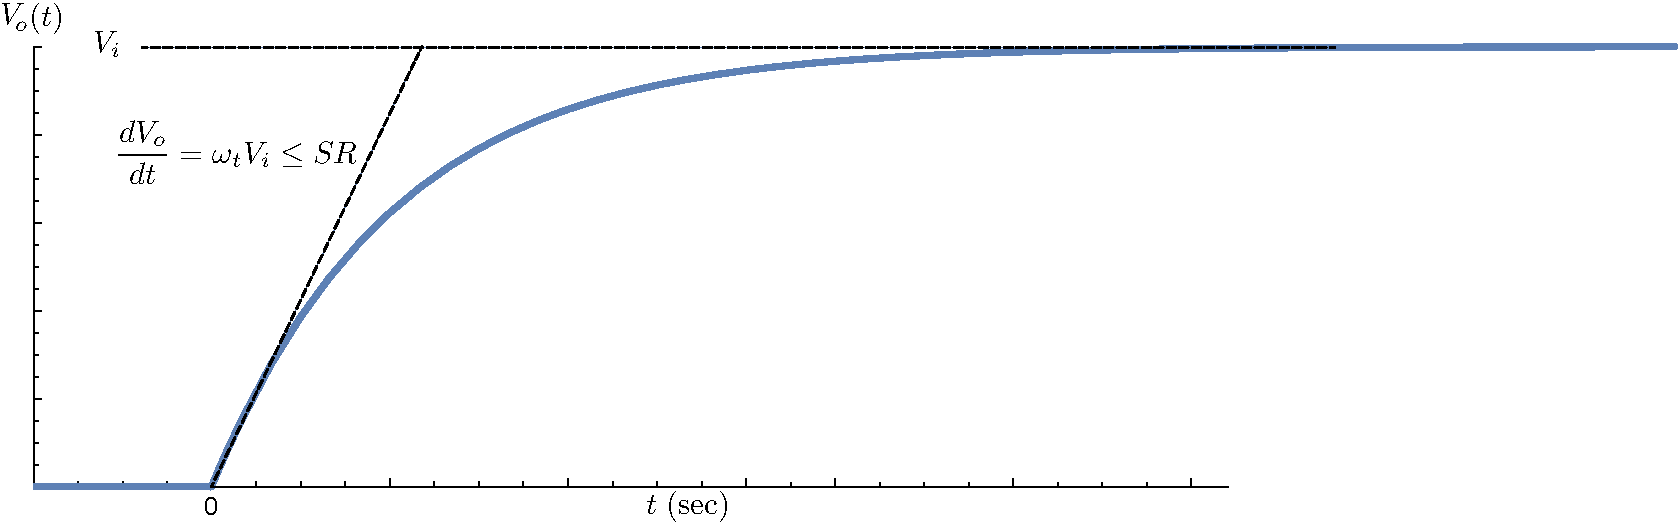
\includegraphics[width=.8\columnwidth]{SR_case2}
\caption{In this example, the slope of the output is lower than the $SR$ limit, and so the output experiences linear settling time rather than SR limiting.}
\label{fig:SR_case2}
\end{figure}
%%%%%%%%%%%%%%%%%%%%%%%%%%%%%%%%%%%%%%%%%%%%
%             SUBSECTION 18.4.3            %
%%%%%%%%%%%%%%%%%%%%%%%%%%%%%%%%%%%%%%%%%%%%
\subsection{Origin of Slew Rate Limit}
%%%%%%%%%%%%%%%%%%%%%%%%%%%%%%%%%%%%%%%%%%%%
%                 FIGURE                   %
%%%%%%%%%%%%%%%%%%%%%%%%%%%%%%%%%%%%%%%%%%%%
\begin{figure}[tb]
\centering
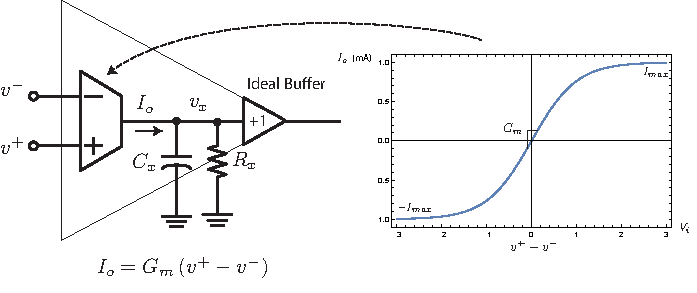
\includegraphics[width=\columnwidth]{opamp_ota_SR}
\caption{The origin of SR limiting can be understood if we examine the internals of an op-amp. If the input OTA $G_m$ stage current clips for large input voltages, a constant current will flow into the internal node of the op-amp, which results in a SR limited constant slope waveform.}
\label{fig:opamp_ota_SR}
\end{figure}

Note that our simple model of an op-amp has a $G_m$ that can in theory supply any current to the internal high-Z node capacitor. In practice, the current will eventually clip (as shown in \emph{Fig.~\ref{fig:opamp_ota_SR}}, causing SR limitation.  Current clipping is similar to voltage clipping. If internal circuits are biased with a constant supply current, they often cannot exceed a certain limit.  This is true of a differential pair that we studied in the last chapter.  If a buffer stage is added to the amplifier, slewing may occur to the finite DC current of the buffer as well.  For the model shown, suppose a large input step is applied so that the OTA current is clipped.  Then the internal node of the amplifier, initially at zero, will ramp at a constant rate due the the constant current supply flowing into a capacitor:
    \begin{equation}
        C_x \frac{dV_x}{dt} = I_{G_m} = \pm I_{max} 
    \end{equation}
In this equation we're ignoring the impact of the large resistor $R_x$ for simplicity.  Since $I_{max}$ is a constant, we see that the rate of change of the output, or the SR at the internal node, is fixed:
    \begin{equation}
        \left.	\frac{dv_x}{dt} \right|_{\text{max}} = \pm \frac{I_{max}}{C_x} 
    \end{equation}
linear settling will resume when the input error voltage reduces (due to feedback) and the $G_m$ enters the linear range.
%%%%%%%%%%%%%%%%%%%%%%%%%%%%%%%%%%%%%%%%%%%%
%             SUBSECTION 18.4.4            %
%%%%%%%%%%%%%%%%%%%%%%%%%%%%%%%%%%%%%%%%%%%%
\subsection{Full-Power Bandwidth}
%%%%%%%%%%%%%%%%%%%%%%%%%%%%%%%%%%%%%%%%%%%%
%                 FIGURE                   %
%%%%%%%%%%%%%%%%%%%%%%%%%%%%%%%%%%%%%%%%%%%%
\begin{figure}[tb]
\centering
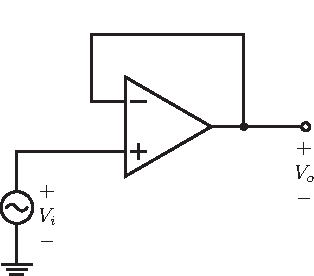
\includegraphics[scale=1]{opamp_unitygain}
\caption{When a sinusoidal voltage is applied to a unity-gain amplifier, if the slope of the input waveform is sufficiently large, the output waveform will be distorted.  The full-power bandwidth is the largest frequency that the amplifier can process linearly without SR limiting.}
\label{fig:opamp_unitygain_fig}
\end{figure}
%%%%%%%%%%%%%%%%%%%%%%%%%%%%%%%%%%%%%%%%%%%%
Now let's suppose we drive our amplifier with a sinusoidal signal, shown in \emph{Fig.~\ref{fig:opamp_unitygain_fig}}.  Since the follower is a  unity-gain amplifier, we expect the output to be given by:
    \begin{equation} 
        V_o = V_i \sin\omega t 
    \end{equation}
The rate of change of the output must be less than the slew-rate:
    \begin{equation}
        \frac{dV_o}{dt} = V_i \omega \cos\omega t 
    \end{equation}
Since $|\cos(\omega t)| \le 1$, the maximum slope is given by
    \begin{equation}
        \left. \frac{dV_o}{dt} \right|_{\text{max}} = V_i \omega 
    \end{equation}
The full-power bandwidth is known as the frequency at which the SR-limited distortion starts to occur for an output sinusoid with maximum rated output voltage, $V_{o,max}$:
    \begin{equation}
        \omega_{max} V_{o,max} = SR
    \end{equation} 
Interestingly, this frequency may be much lower than the unity gain frequency (linear bandwidth limit) of the amplifier:
    \begin{equation} 
        f_{max} = \frac{SR}{2\pi V_{o,max}} 
    \end{equation}
Notice again that the frequency $f_{max}$ is a function of the output amplitude.  If the amplitude of the signal is lowered, then the $SR$ limit can be avoided.  In other words, we can find the smallest amplitude such that the amplifier always settles linearly by equation $f_{max}$ with the unity-gain frequency.
%%%%%%%%%%%%%%%%%%%%%%%%%%%%%%%%%%%%%%%%%%%%%%%%%%%%%%%%%%%%%%%%%%%%%%%%%%%%%%%%%%%%%%%%
%%%%%%%%%%%%%%%%%%%%%%%%%%%%%%%%%%%%%%%%%%%%%%%%%%%%%%%%%%%%%%%%%%%%%%%%%%%%%%%%%%%%%%%%
%                                   SECTION 18.5                                       %
%%%%%%%%%%%%%%%%%%%%%%%%%%%%%%%%%%%%%%%%%%%%%%%%%%%%%%%%%%%%%%%%%%%%%%%%%%%%%%%%%%%%%%%%
%%%%%%%%%%%%%%%%%%%%%%%%%%%%%%%%%%%%%%%%%%%%%%%%%%%%%%%%%%%%%%%%%%%%%%%%%%%%%%%%%%%%%%%%
\section{Noise and Distortion}
%%%%%%%%%%%%%%%%%%%%%%%%%%%%%%%%%%%%%%%%%%%%
%             SUBSECTION 18.5.1            %
%%%%%%%%%%%%%%%%%%%%%%%%%%%%%%%%%%%%%%%%%%%%
\subsection{Op-Amp Distortion}
%%%%%%%%%%%%%%%%%%%%%%%%%%%%%%%%%%%%%%%%%%%%
%                 FIGURE                   %
%%%%%%%%%%%%%%%%%%%%%%%%%%%%%%%%%%%%%%%%%%%%
\begin{figure}[tb]
\centering
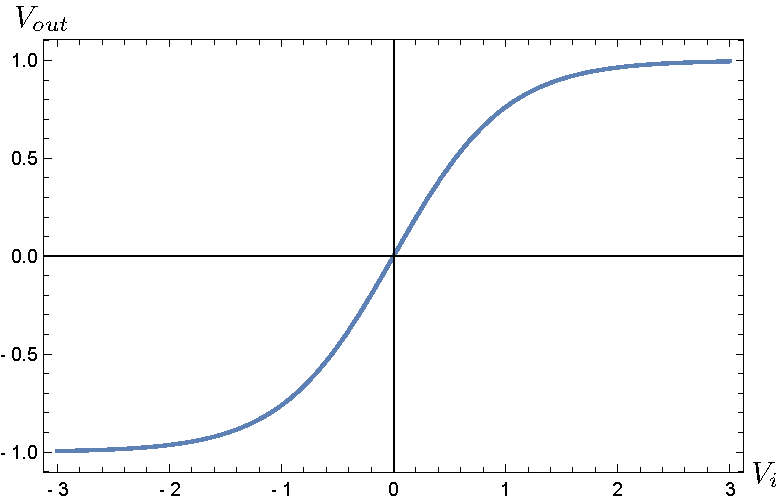
\includegraphics[width=.75\columnwidth]{vtanh}
\caption{The typical input-output relationship is "S" shaped because of various limits that eventually clip the waveform.}
\label{fig:vtanh}
\end{figure}
%%%%%%%%%%%%%%%%%%%%%%%%%%%%%%%%%%%%%%%%%%%%
%                 FIGURE                   %
%%%%%%%%%%%%%%%%%%%%%%%%%%%%%%%%%%%%%%%%%%%%
\begin{figure}[tb]
\centering
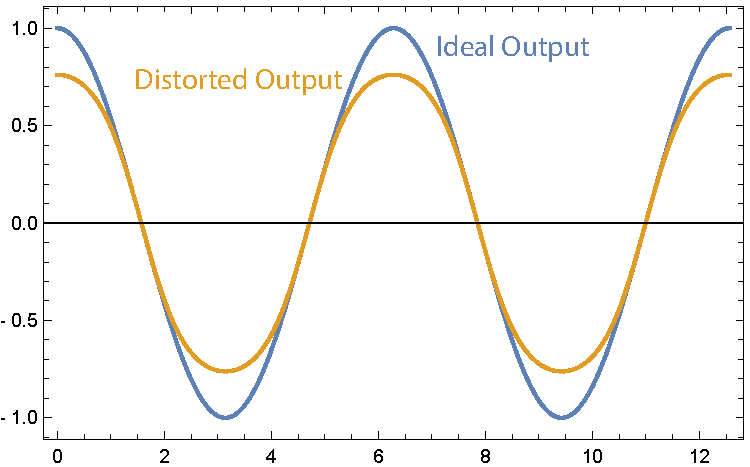
\includegraphics[width=.75\columnwidth]{vdisto}
\caption{When a sinusoidal waveform experiences non-linearity as shown in \emph{Fig.~\ref{fig:vtanh}}, the output waveform is no longer a pure tone, but contains harmonics, that lead to distortion.}
\label{fig:vdisto}
\end{figure}
%%%%%%%%%%%%%%%%%%%%%%%%%%%%%%%%%%%%%%%%%%%%
As we have seen, the op-amp output signal has several sources of distortion arising from clipping, slewing, and even bandwidth limits if the phase of the signal introduces a non-constant group delay in the frequency response.  Another source of distortion is that the gain is signal dependent.  In other words, the input-output curve is not a perfect straight line but has curvature ("S" shaped for example), as shown in \emph{Fig.~\ref{fig:vtanh}}.  We already encountered this when we derived the large signal transfer function of the MOS differential pair (see \emph{Fig.~\ref{fig:Diff_amp_large.pdf}}), and of course all the transistors we have studied have a non-linear $I$-$V$ and $C$-$V$ curve.  This leads to harmonic and intermodulation distortion, a topic we will cover in detail in other courses, such as a communication circuits or advanced analog circuits course.  As a simple example, in \emph{Fig.~\ref{fig:vdisto}}, the ideal sinusoidal output is distorted due to harmonics of the waveform.  Harmonics are generated due to non-linearity.  For example, if we model a small portion of the $I$-$V$ curve with a Taylor series expansion, we have
    \begin{equation}
        I = a_1 V_i + a_2 V_i^2 + a_3 V_i^3 + \cdots
    \end{equation}
If you square a sinusoid, you get second harmonic:
    \begin{equation}
        \cos^2(\omega t) = \frac{1}{2} \left(1 + \cos(2 \omega t) \right)
    \end{equation}
and if we cube a sinusoid:
    \begin{equation}
        \cos^3(\omega t) = \cos(\omega t) \cos^2(\omega t) = \frac{1}{2} \left(\cos(\omega t) + \cos(\omega t)\cos(2 \omega t) \right)
    \end{equation}
Using the following identify
    \begin{equation}
        \cos(a) \cos(b) = \frac{1}{2} \left( \cos(a - b) + \cos(a + b) \right) 
    \end{equation}
The cubic can be simplified into a sum of fundamental at a frequency $\omega$ and third harmonic:
    \begin{equation}
        \cos^3(\omega t) =  \frac{3}{4} \cos(\omega t) + \frac{1}{4} \cos(3 \omega t)) 	
    \end{equation}
These harmonics lead to waveform distortion shown in \emph{Fig.~\ref{fig:vdisto}}.  Fortunately, in negative feedback systems, the input voltage swing is small and these harmonics are very small and unnoticeable with the naked eye.  One has to use a very sensitive measurement system, such as a spectrum analyzer, to detect the distortion under normal operating conditions.
%%%%%%%%%%%%%%%%%%%%%%%%%%%%%%%%%%%%%%%%%%%%
%             SUBSECTION 18.5.2            %
%%%%%%%%%%%%%%%%%%%%%%%%%%%%%%%%%%%%%%%%%%%%
\subsection{Op-Amp Noise}
%%%%%%%%%%%%%%%%%%%%%%%%%%%%%%%%%%%%%%%%%%%%
%                 FIGURE                   %
%%%%%%%%%%%%%%%%%%%%%%%%%%%%%%%%%%%%%%%%%%%%
\begin{figure}[tb]
\centering
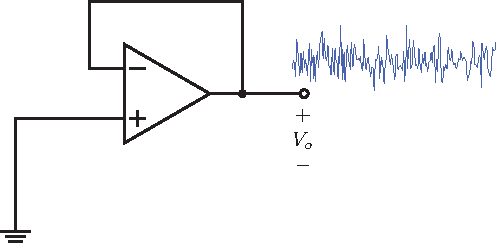
\includegraphics[scale=1]{opamp_unitygain_noise}
\caption{When we short the inputs of an amplifier and examine the output with a sensitive instrument, we find a small random AC signal.  This signal is always present and depends on the temperature of the setup due to the thermodynamic origin.}
\label{fig:opamp_unitygain_noise_fig}
\end{figure}
%%%%%%%%%%%%%%%%%%%%%%%%%%%%%%%%%%%%%%%%%%%%
Imagine that you short circuit the input of your op-amp as shown in \emph{Fig.~\ref{fig:opamp_unitygain_noise_fig}}. In addition to offset voltage, you would also observe a random fluctuation of the output signal.  The signal is very small and it might be below the resolution limits of the oscilloscope, but a more sensitive instrument such as a spectrum analyzer clearly shows this noise.  The noise tends to be flat in spectrum and for this reason it's often called "white noise".  While we sometimes call interference signals noise, here we are referring to a random signal originating from thermodynamic properties of the transistor, rather than human made noise that couples into the circuit.   Since it's a random signal, it's characterized by its statistical properties, such as the standard deviation of the signal.  
%%%%%%%%%%%%%%%%%%%%%%%%%%%%%%%%%%%%%%%%%%%%
Op-amps, like all amplifiers, have noise.  We model the noise in the same way that we modeled offset voltages, as input voltages and/or currents as shown in \emph{Fig.~\ref{fig:opamp_noise}}.  Unlike offset voltages, these are AC signals that are characterized in the frequency domain.  Since the signal is usually flat with frequency, the noise spectral density, or the amount of noise power per unit bandwidth, is stated in datasheets.  To get the voltage or current noise, you must integrate the noise over the bandwidth of interest.  If the noise has a flat spectrum, you multiply the noise power density by the bandwidth of interest (approximately the bandwidth of the amplifier) and take the square root.  This is why you will often see voltage and current noise specified in units of square root of hertz.
%%%%%%%%%%%%%%%%%%%%%%%%%%%%%%%%%%%%%%%%%%%%
In addition to active devices like transistors, resistors also generate noise due to the random motion of carriers (electrons) in the solid.  At any given time instant, the number of carriers moving "left" versus "right" is not equal, and so the device is conducting current. This is why the current is very small, because it's the imbalance of carrier motion, and why the signal is an AC signal with current going positive and then almost immediately going negative with very high rate (frequency).  The noise current is proportional to the temperature $T$ because it's due to the random thermal motion of carriers.  In a resistor, it can be shown that the current takes on a value of
    \begin{equation}
        i_R = \sqrt{4 k T \frac{1}{R} \Delta f} 
    \end{equation}
where $k$ is Boltzmann's constant, and $\Delta f$ is the bandwidth of interest.   Using a Norton to Thévenin transformation, we can state this as a noise voltage of value
    \begin{equation}
        v_R = \sqrt{4 k T R \Delta f} 
    \end{equation}
A handy rule of thumb to remember is that a 1k$\Omega$ resistor has an integrated noise of 4$\mu$V for a 1 MHz of bandwidth.   Since resistors are used in the feedback of amplifiers, they also contribute noise. Low noise designs therefore favor small resistors in feedback.  In the design of signal processing chains, we must always ensure that the minimum signal level is much larger than noise level, otherwise the quality of the signal, or the signal-to-noise ratio (SNR) degrades.
%%%%%%%%%%%%%%%%%%%%%%%%%%%%%%%%%%%%%%%%%%%%
%                 FIGURE                   %
%%%%%%%%%%%%%%%%%%%%%%%%%%%%%%%%%%%%%%%%%%%%
\begin{figure}[tb]
\centering
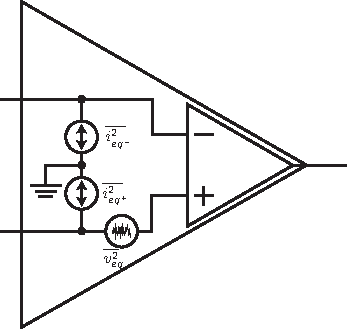
\includegraphics[scale=1]{opamp_noise}
\caption{The noise of an op-amp can be modeled by a noiseless op-amp and internal input voltage and current noise sources as shown.}
\label{fig:opamp_noise}
\end{figure}
%%%%%%%%%%%%%%%%%%%%%%%%%%%%%%%%%%%%%%%%%%%%%%%%%%%%%%%%%%%%%%%%%%%%%%%%%%%%%%%%%%%%%%%%
%%%%%%%%%%%%%%%%%%%%%%%%%%%%%%%%%%%%%%%%%%%%%%%%%%%%%%%%%%%%%%%%%%%%%%%%%%%%%%%%%%%%%%%%
%                                   SECTION 18.6                                       %
%%%%%%%%%%%%%%%%%%%%%%%%%%%%%%%%%%%%%%%%%%%%%%%%%%%%%%%%%%%%%%%%%%%%%%%%%%%%%%%%%%%%%%%%
%%%%%%%%%%%%%%%%%%%%%%%%%%%%%%%%%%%%%%%%%%%%%%%%%%%%%%%%%%%%%%%%%%%%%%%%%%%%%%%%%%%%%%%%
\section{Datasheets}
Now that we have covered nearly all aspects of real op-amps, it's fun to look at some typical datasheets of practical amplifiers and to appreciate all of the specifications.  Let's take the Analog Devices ADA4891 CMOS op-amp, summarized in \emph{Fig.~\ref{fig:adi_datasheet.png}}.  This is advertised as a general purpose high speed op-amp.  It has a gain bandwidth product of 240 MHz, a slew rate SR of 170V/$\mu$s, a DC offset of 2mV and an open-loop DC gain of 66 dB.  Being a CMOS op-amp, the input impedance is very large at 5G$\Omega$, and it has an input common mode range of $-V_s - 0.3$V to $+V_s - 0.8$V ($V_s$ is the supply voltage).  The common-mode rejection ratio (CMRR) is 88 dB.  Take a look at the table and make sure you understand most, if not all, of the specifications!
%%%%%%%%%%%%%%%%%%%%%%%%%%%%%%%%%%%%%%%%%%%%
%                 FIGURE                   %
%%%%%%%%%%%%%%%%%%%%%%%%%%%%%%%%%%%%%%%%%%%%
\begin{figure}[tb]
\centering
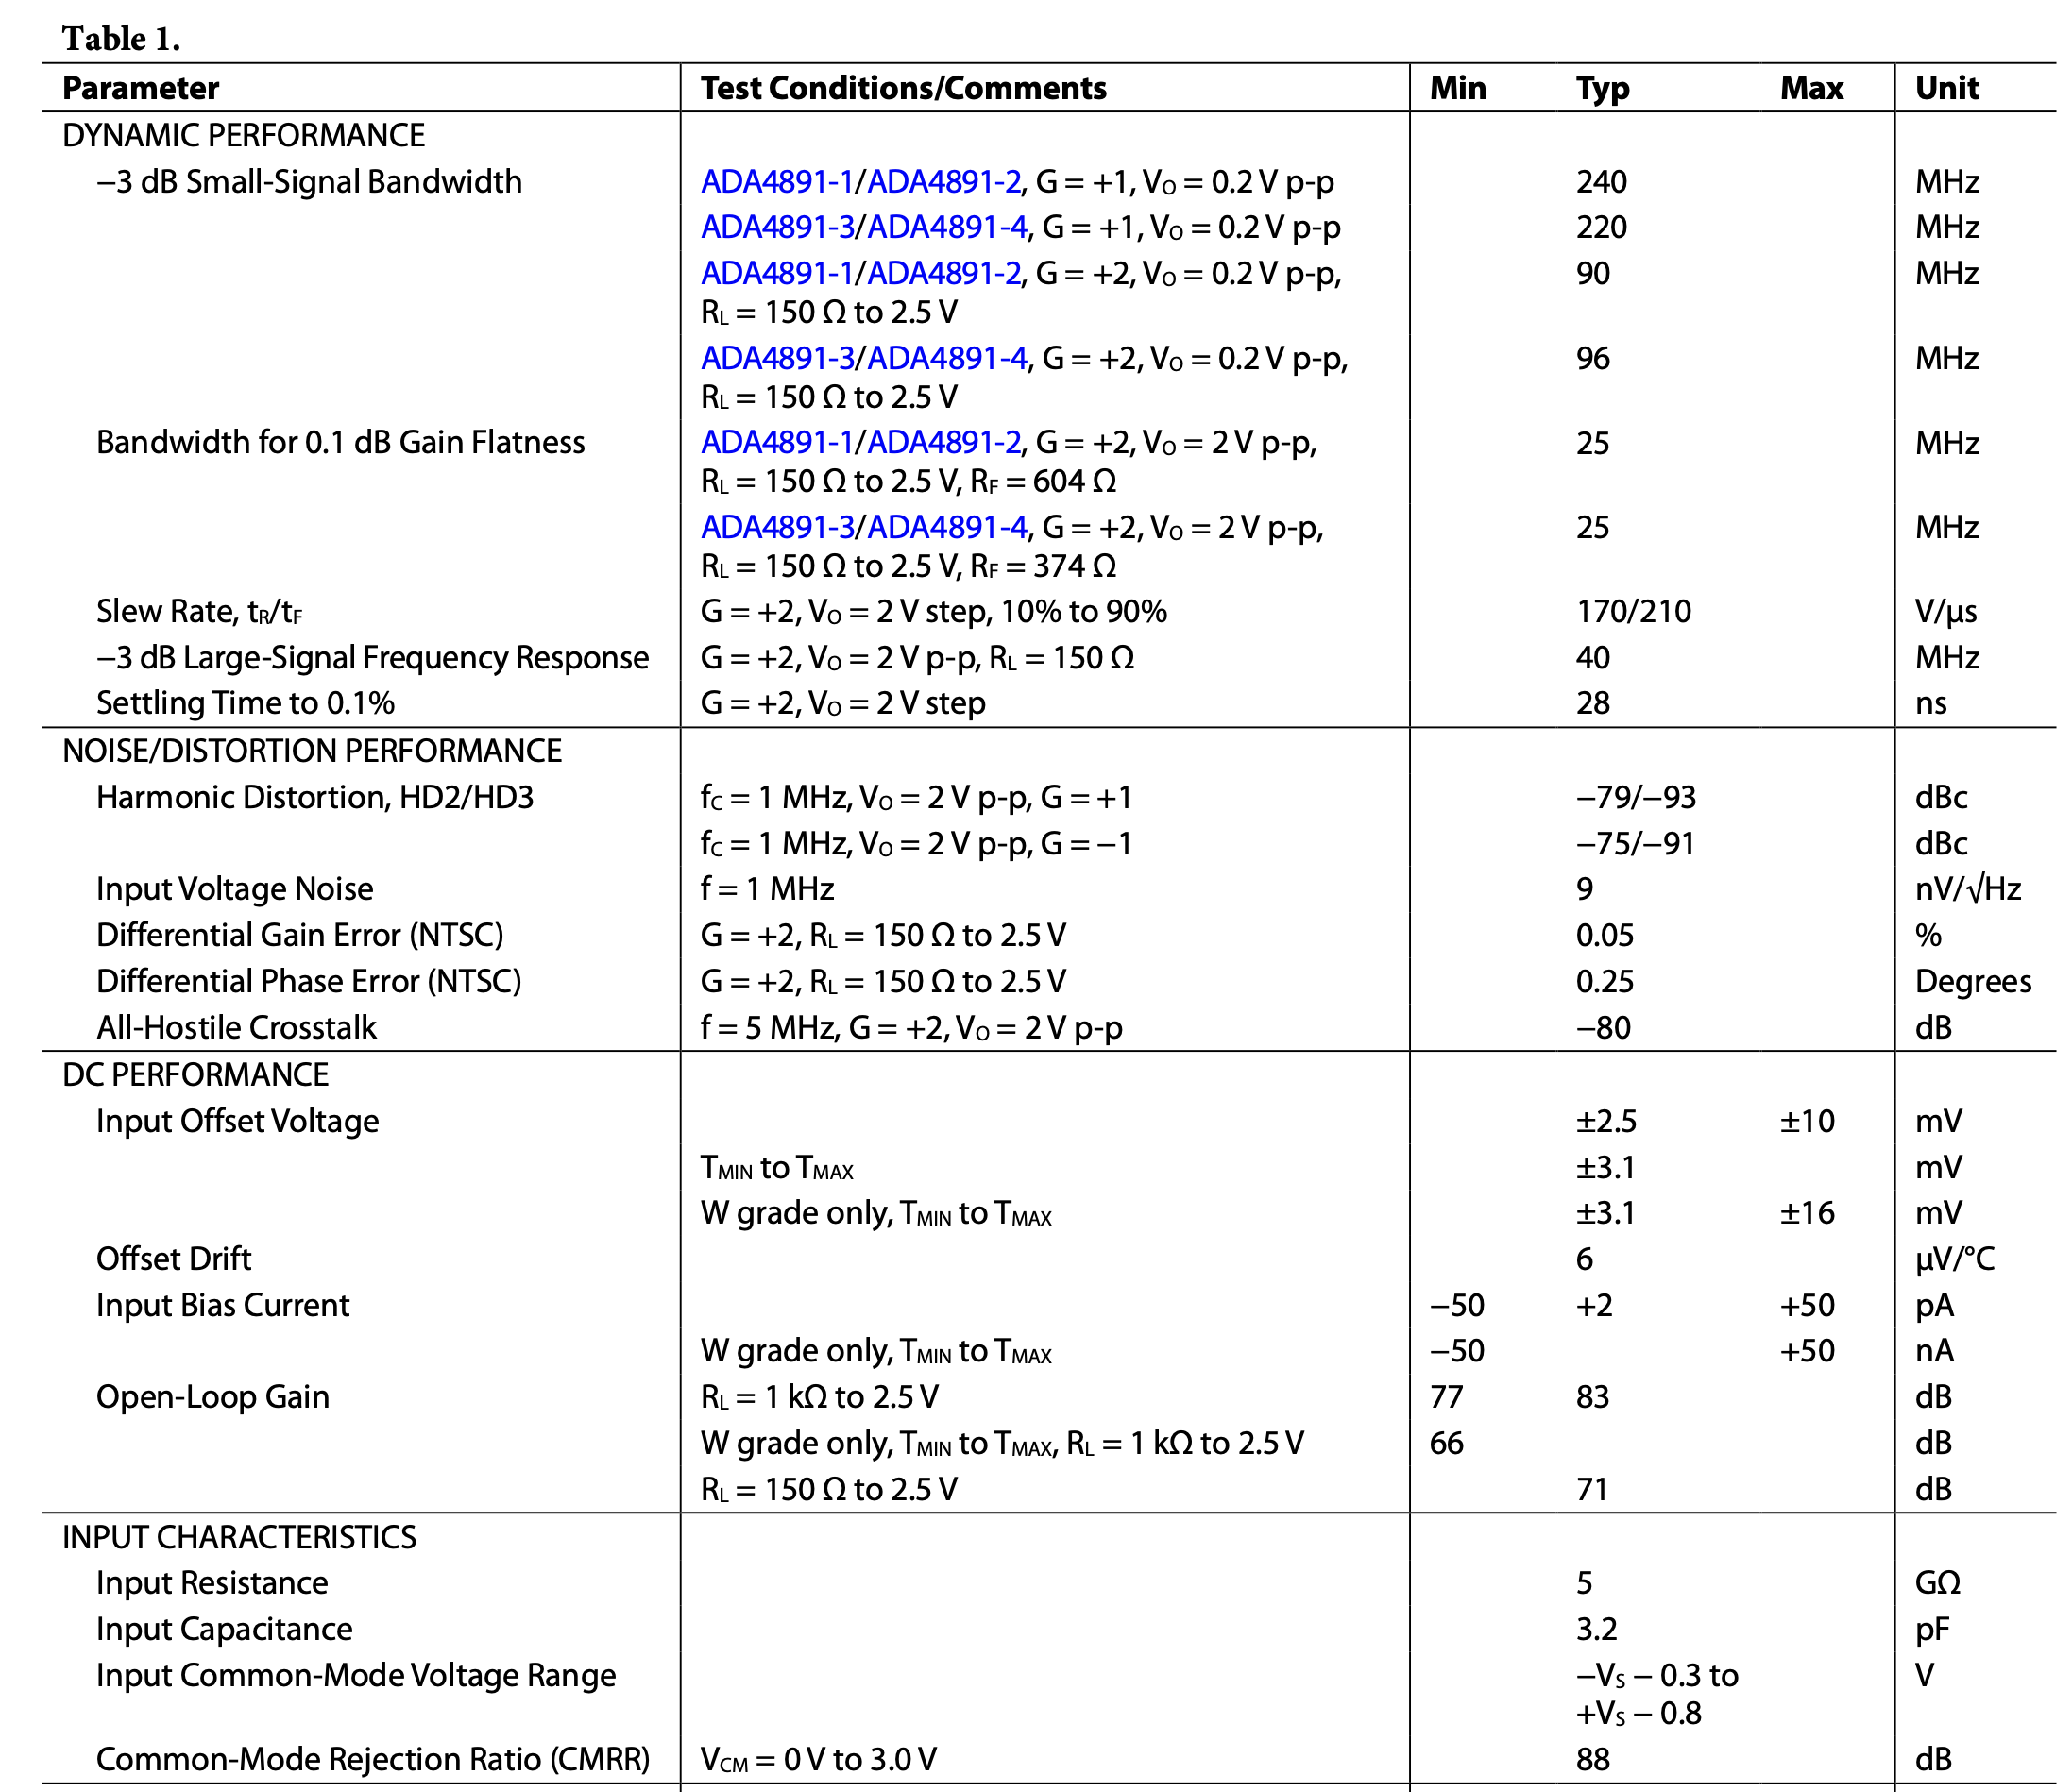
\includegraphics[width=1\columnwidth]{ada4891_datasheet_table.png}
\caption{The datasheet for the ADA4891 op-amp.  See \url{https://www.analog.com/media/en/technical-documentation/data-sheets/ADA4891-1_4891-2_4891-3_4891-4.PDF}.}
\label{fig:adi_datasheet.png}
\end{figure}
%%%%%%%%%%%%%%%%%%%%%%%%%%%%%%%%%%%%%%%%%%%%
It's important to realize that there are hundreds of op-amps that suit different applications.  For example, in \emph{Fig.~\ref{fig:opamp_table.png}}, we show a table of op-amps from Analog Devices that are sorted by the $GBW$ product.  The fastest op-amps have amazing unity gain frequencies (3.8 GHz) and very high slew rates approaching 1GV/s.  The cost is power consumption, which is 10's of mA.  On the other end of the spectrum, if we look for very low power op-amps, suitable for sensor or IoT applications, we also find amplifiers with amazing specifications, such as sub micro-amp current consumption, but at a severe penalty of speed, both in $GBW$ product and in slew rate.  
%%%%%%%%%%%%%%%%%%%%%%%%%%%%%%%%%%%%%%%%%%%%
%                 FIGURE                   %
%%%%%%%%%%%%%%%%%%%%%%%%%%%%%%%%%%%%%%%%%%%%
\begin{figure}[tb]
\centering
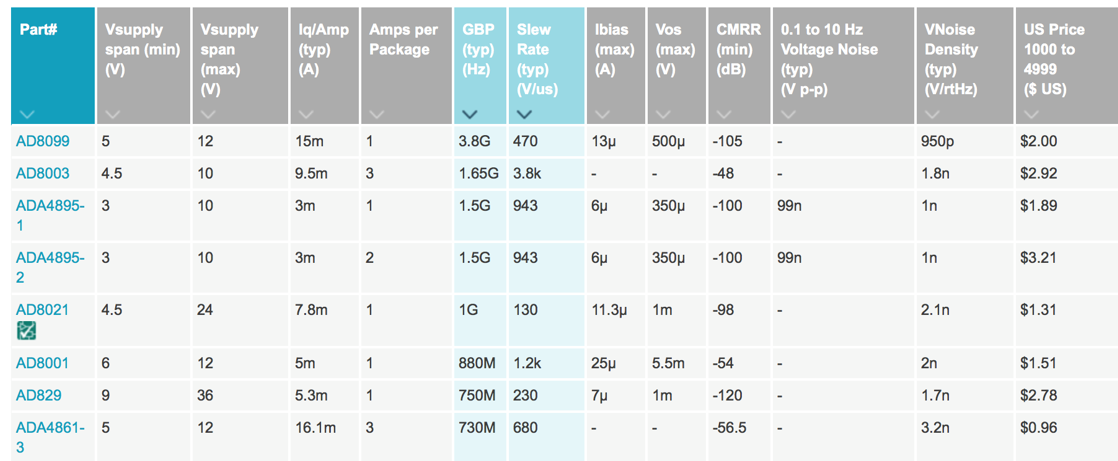
\includegraphics[width=\columnwidth]{opamp_table.png}
\caption{A list of op-amps offered by Analog Devices, sorted by gain-bandwidth product.  These are the highest bandwidth and highest slew rate amplifiers.  See \url{https://www.analog.com/en/products/amplifiers/operational-amplifiers.html}.} \label{fig:opamp_table.png}
\end{figure}
%%%%%%%%%%%%%%%%%%%%%%%%%%%%%%%%%%%%%%%%%%%%
%                 FIGURE                   %
%%%%%%%%%%%%%%%%%%%%%%%%%%%%%%%%%%%%%%%%%%%%
\begin{figure}[tb]
\centering
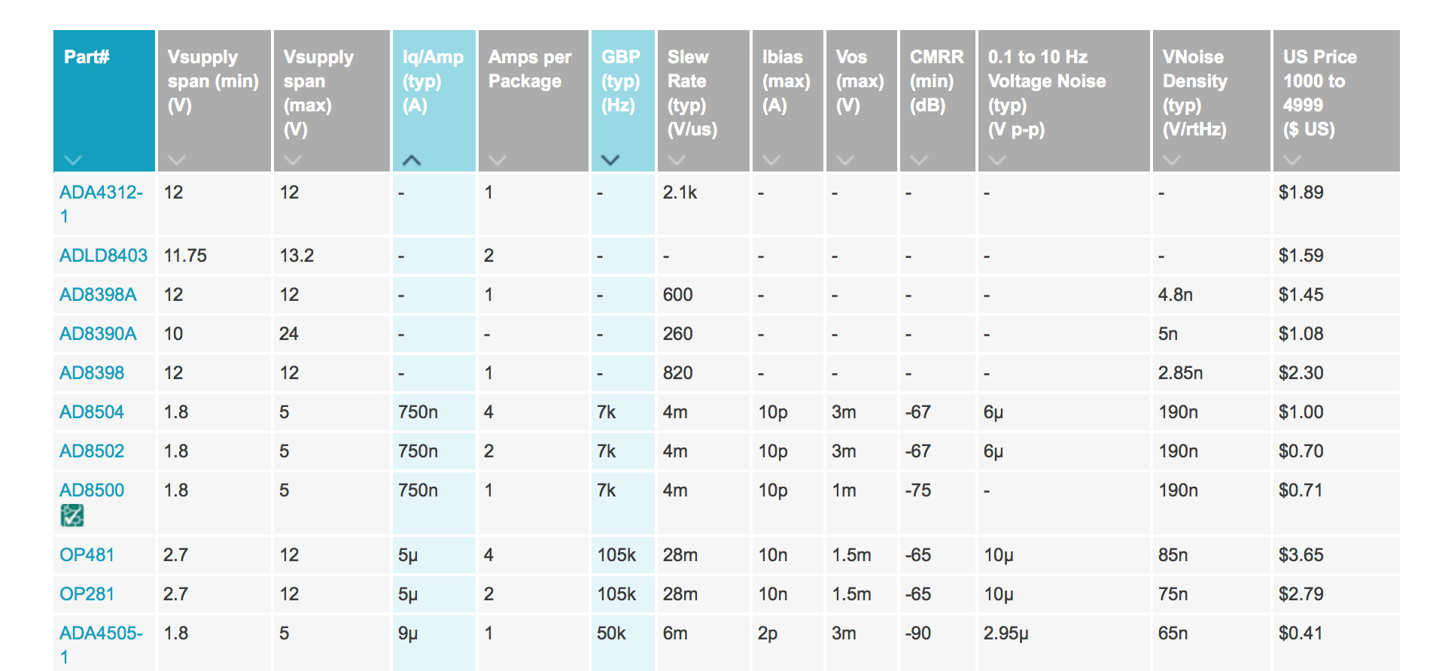
\includegraphics[width=\columnwidth]{opamp_lowpower.png}
\caption{A list of op-amps offered by Analog Devices, sorted by power consumption.  These are the lowest power amplifiers suitable for IoT and sensor applications.  See \url{https://www.analog.com/en/products/amplifiers/operational-amplifiers.html}.} \label{fig:opamp_lowpower.png}
\end{figure}
%%%%%%%%%%%%%%%%%%%%%%%%%%%%%%%%%%%%%%%%%%%%
\newpage
%%%%%%%%%%%%%%%%%%%%%%%%%%%%%%%%%%%%%%%%%%%%%%%%%%%%%%%%%%%%%%%%%%%%%%%%%%%%%%%%%%%%%%%%
%%%%%%%%%%%%%%%%%%%%%%%%%%%%%%%%%%%%%%%%%%%%%%%%%%%%%%%%%%%%%%%%%%%%%%%%%%%%%%%%%%%%%%%%
%                                 SECTION 18.7                                         %
%%%%%%%%%%%%%%%%%%%%%%%%%%%%%%%%%%%%%%%%%%%%%%%%%%%%%%%%%%%%%%%%%%%%%%%%%%%%%%%%%%%%%%%%
%%%%%%%%%%%%%%%%%%%%%%%%%%%%%%%%%%%%%%%%%%%%%%%%%%%%%%%%%%%%%%%%%%%%%%%%%%%%%%%%%%%%%%%%
\section{Chapter Summary}
In this chapter we ...
